\section{Contract 3: Bloom filter}

While variant 1 of the smart contract is space-inefficient and variant 2 needs additional infrastructure, variant 3 is an attempt to strike a balance. It is a standalone contract that solves the scalability issue by using a bloom filter.

A bloom filter is a probabilistic data structure that is very space efficient. In the context of large amounts of IP addresses, it can be tested if an IP address has been inserted into the bloom filter beforehand with constant space requirements. False positives are possible, false negatives are not.

This variant is space-efficient and the logic is self-contained, however perfect accuracy cannot be guaranteed anymore. Also, additional parameters like a blacklist/whitelist flag, expiration dates, ip boundaries can not be stored in a bloom filter, as it is impossible to fully retrieve the information that the bloom filter was fed.

It is however possible to store additional information in the contract, and use multiple contracts if the parameters differ for reports.

No implementation of a bloom filter in Solidity could be found online, therefore the approach taken to implement this variant was to convert one of the countless examples written in other programming languages into Solidity.

One part of a bloom filter is the hash function that takes any string and converts it into a fixed-length hash. The other part is managing the store, and exposing interfaces for adding entries and checking if an entry has been added.

Different hash functions are available and the choice of the hash function influences the properties of the bloom filter, mainly accuracy and speed. A bloom filter becomes more accurate if the hash function it uses produces more uniform hashes. However, usually more uniform results also means slower hashing.

\subsection{Hashing function}

The hashing part is the more complex code to convert to Solidity, since hashing functions use big numbers and bit-shifting to generate their hashes, which both are very prone to differences in different environments.

In an first attempt, the popular hashing library \texttt{imurmurhash} \cite{imurmur} was taken and rewritten in Solidity as close as possible. This library is using the \texttt{\textgreater{}\textgreater{}\textgreater} (logical right shift) operator which is absent in Solidity. By using a \texttt{\textgreater{}\textgreater} (arithmetic right shift) operator instead, the hashes could not be reproduced. It also generated big numbers in the process whose behavor was inconsistent between Ethereum VM and Javascript environments.
When later using the ported hash function in a bloom filter, it would return many false positives\footnote{A test case showing the false positive is available under \texttt{test/hash-function.js} in the project files.}.

In an second attempt, the \texttt{bloomfilter.js} \cite{bloomfilterjs} library was ported to Solidity as close as possible. This library uses the Fowler-Noll-Vo hash function instead. The commit history shows that it had once worked without the \texttt{\textgreater{}\textgreater{}\textgreater} operator, but that operator was added later. Yet, the Solidity implementation did still not yield the same hashes for the same input as the Javascript equivalent of the code. By testing subfunctions of the hash function, it was discovered that the inconsistency is caused by bug numbers. In one hash operation, the statement \texttt{2166136261 \textasciicircum{} 65 \& 0xff} would be executed. It is easily verifiable that this expression evaluates to \texttt{-2128831100} in Javascript and to \texttt{2166136196} in Solidity Version 0.4.9.

This difference results because Solidity uses types for numbers such as \texttt{int}, while Javascript only supports floating-point math. With the different hashes being generated, the contract that resulted from the second attempt also led to false positives. \footnote{A test case showing the false positive is available under \texttt{test/hash-function-2.js} in the project files.}

Porting existing hash functions to Solidity provides great challenges. For the third attempt, bloom filter implementations were searched that used one of the hash functions already implemented in Solidity. Two hashing algorithm functions are globally available in every Solidity contract, \texttt{sha256()} and \texttt{sha3()}. For the third attempt, a 'Simple Bloom Filter' \cite{SimpleBloomFilter} code snippet from Github was used as the basis for the smart contract.

This third attempt proved successful as the SHA-256 hashes are reproducible and false positives did not occur anymore. The smart contract that resulted from this attempt has also the most concise and easiest to read code.

\subsection{Hashing parameters}

Instead of only hashing an input value once, it usually is hashed multiple times. This reduces the chance of collision \cite{MultipleHashes}. The amount of hash iterations is also variable. In this simple bloom filter, additional hashes beyond the first one are just bit-shifts of the first hash.

The bloom filter takes two parameters: numbers of bits in the filter and number of hash functions. 

The bigger the amount of the array items and the bigger the amount of the hash iterations, the more accurate a bloom filter gets. The default parameters of the Python bloom filter were an array size of 1024 bytes and 13 hash iterations. \cite{SimpleBloomFilter}.

In Solidity however, this configuration would raise an 'out of gas' error when adding a string to the filter. 
The maximum amount of gas (also called gas limit) that can be spent on a transaction is 3,141,592 (pi million). Since every node in the network needs to download every transaction, there is an artificial cap on how computationally expensive a transaction may be.

By decreasing the array size to 512 bytes, the cost stays below the gas limit and the bloom filter works. 
Testing different values determined that an array size of 836 bytes is the maximum before this specific contract would not be able to have a transaction executed. However this thesis continues with the assumption of a 512 byte array size to stay well below the gas limit \textemdash \ this way more features can be added without hitting the gas threshold.

\subsection{Accuracy}

Given a number of items that are indexed, and a number of hash functions, the ideal array size and number of hash functions can be calculated. According to http://hur.st \cite{BloomfilterAccuracy}, given $n$ = number of items in the filter and $p =$ probability of false positives, the number of bits in the filter $m$ can be calculated using equation \ref{eq:m} and the number of hash functions $k$ using equation \ref{eq:k}. 

\begin{equation}
m = \lceil\frac{n * log(p)}{ln(\frac{1.0}{2.0 ^{ln(2)}})}\rceil
\label{eq:m}
\end{equation}

\begin{equation}
k = \lfloor ln(2) * m / n) \rceil
\label{eq:k}
\end{equation}

For example: Given that the magnitude of DDoS attacks is in the millions (n = 1'000'000) and assuming that a 5\% chance of false positives is good enough (p = 0.05), an array size of 14357134 bits (1.71 MB) and 4 hash functions will do.

Solving equation \ref{eq:m} for $p$ gives equation \ref{eq:p}.

\begin{equation}
p = e^{\frac{{m \cdot ln(\frac{1}{2^{ln(2)}})}}{n}}
\label{eq:p}
\end{equation}

The probability of at least one false positive is shown in table \ref{table:Probability} and figure 4.1. It assumes the number of \textbf{bits} in the filter is 4'096 ($512\ bytes \cdot 8$).

\begin{table}[ht]
\begin{minipage}[b]{.45\textwidth}
        \begin{tabular}{r | r}
            \hline
            IP addresses ($n$) & Probability \\ \hline
            1 & $10^{-855}$ \\ \hline
            10 & $10^{-86}$ \\ \hline
            100 & $10^{-9}$ \\ \hline
            1'000 & 0.14 \\ \hline
            10'000 & 0.82 \\ \hline
            100'000 & 0.98 \\ \hline
            1'000'000 & 0.998 \\ \hline
            10'000'000 & 0.9998 \\ \hline
        \end{tabular}
            \caption{Probability of false positives, using equation \ref{eq:p} and $m = 4'096$}
            \label{table:Probability}
\end{minipage}
\hspace{.1\textwidth}
\begin{minipage}[b]{.45\textwidth}
        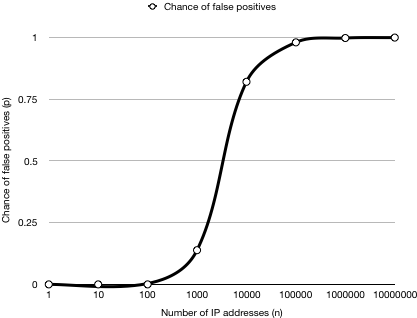
\includegraphics[width=1\textwidth]{v3-chance.png}
        \label{fig:Probability}
        \captionof{figure}{Probability of false positives, using data from Table \ref{table:Probability} (logarithmic scale)}
\end{minipage}
\end{table}

The bloom filter does have a false positive chance of under 1\% for up to 425 IP addresses. Inserting more IP addresses after that decreases the accuracy of the bloom filter dramatically. With 1'000 insertions, variant 3 would lead to 14\% of legimitate traffic being blocked. With 3'000 insertions, over half of the legitimate traffic would be falsly blocked.

With the gas limit constaint in place and the probabilities in mind, it is recommended to use more than one contract if the probability of false positives would be higher than acceptable otherwise. The acceptable probability of false positives is individual for each user.

\subsection{State management and interface}

A bloom filter creates a fixed length array that initially only contains zeroes.
\definecolor{dkgreen}{rgb}{0,0.6,0}
\definecolor{gray}{rgb}{0.5,0.5,0.5}
\definecolor{mauve}{rgb}{0.58,0,0.82}

\lstset{frame=tb,
  language=Java,
  aboveskip=3mm,
  belowskip=3mm,
  showstringspaces=false,
  columns=flexible,
  basicstyle={\small\ttfamily},
  numbers=none,
  numberstyle=\tiny\color{gray},
  keywordstyle=\color{blue},
  commentstyle=\color{dkgreen},
  stringstyle=\color{mauve},
  breaklines=true,
  breakatwhitespace=true,
  tabsize=3
}

\lstinputlisting{snippets/contract-3-constructor.sol}


When adding an entry, it gets hashed and some items in the array get bit-shifted from '0' to '1'. The algorithm is taken from the original Python implementation \cite{SimpleBloomFilter}.

\definecolor{dkgreen}{rgb}{0,0.6,0}
\definecolor{gray}{rgb}{0.5,0.5,0.5}
\definecolor{mauve}{rgb}{0.58,0,0.82}

\lstset{frame=tb,
  language=Java,
  aboveskip=3mm,
  belowskip=3mm,
  showstringspaces=false,
  columns=flexible,
  basicstyle={\small\ttfamily},
  numbers=none,
  numberstyle=\tiny\color{gray},
  keywordstyle=\color{blue},
  commentstyle=\color{dkgreen},
  stringstyle=\color{mauve},
  breaklines=true,
  breakatwhitespace=true,
  tabsize=3
}

\lstinputlisting{snippets/contract-3-add.sol}


For testing whether an IP address has been inserted, the input string gets hashed again and the same positions in the array are calculated. If all the values at the array positions are 1's, the bloom filter assumes the string has been inserted before (of course false positives are possible).


\definecolor{dkgreen}{rgb}{0,0.6,0}
\definecolor{gray}{rgb}{0.5,0.5,0.5}
\definecolor{mauve}{rgb}{0.58,0,0.82}

\lstset{frame=tb,
  language=Java,
  aboveskip=3mm,
  belowskip=3mm,
  showstringspaces=false,
  columns=flexible,
  basicstyle={\small\ttfamily},
  numbers=none,
  numberstyle=\tiny\color{gray},
  keywordstyle=\color{blue},
  commentstyle=\color{dkgreen},
  stringstyle=\color{mauve},
  breaklines=true,
  breakatwhitespace=true,
  tabsize=3
}

\lstinputlisting{snippets/contract-3-test.sol}


\subsection{IPv6 format ambiguity consideration}

A IPv6 address can be formatted in more than one way. \cite{RFC4291I66} For instance, leading zeroes in one block can, but don't have to, be omitted. Also, multiple subsequent blocks containing only zeroes can, but don't have to be replaced by two colons.
For example, \texttt{0000:0000:0000:0000:0000:ffff:2e65:6095} can also be formatted as
\path{0:0:0:0:0:ffff:2e65:6095} or even as \texttt{::ffff:2e65:6095}. Passing to the hash function the same IP address, but in different formats, will result in vastly different hashes, assuming an uniform hash function.

To prevent false negatives, the possibility of multiple representations per IP addresses has to be eliminated. Therefore, it makes sense to forbid shorthand notations as well as IPv4-in-IPv6 notations such as \texttt{::ffff:46.101.96.149} and any other alternative notations that RFC 4291 \cite{RFC4291I66} mentions.
This does not result in higher storage costs, as a SHA256 hash is always only 256 bits long.

